\documentclass[12pt]{article}
\usepackage[margin=2cm]{geometry}
\usepackage{titling}
\usepackage{graphicx}
\usepackage{float}
\usepackage[hidelinks]{hyperref}
\usepackage[italian]{babel}
\usepackage{subcaption}

\setlength\parindent{0pt}
\setlength{\parskip}{1em}
\setlength{\droptitle}{-2cm}

\title{Istruzioni d'uso TableFootballPlus}
\author{Università della Svizzera Italiana}
\date{Versione \today}


\begin{document}
\maketitle
\tableofcontents
\newpage

\section{Montaggio}

	\subsection{Tavolo}
	
		Per assemblare il tavolo, avvitare i piedi (1) e posizionare le quattro gambe (2) nei rispettivi angoli; dopodiché inserire la barra stabilizzatrice (3) e fissare le gambe tramite le quattro viti (4). Assicurarsi di tirare completamente le viti e, se necessario, aggiustare l'inclinazione del tavolo tramite i piedini regolabili.

		\begin{figure}[H]
				\centering
                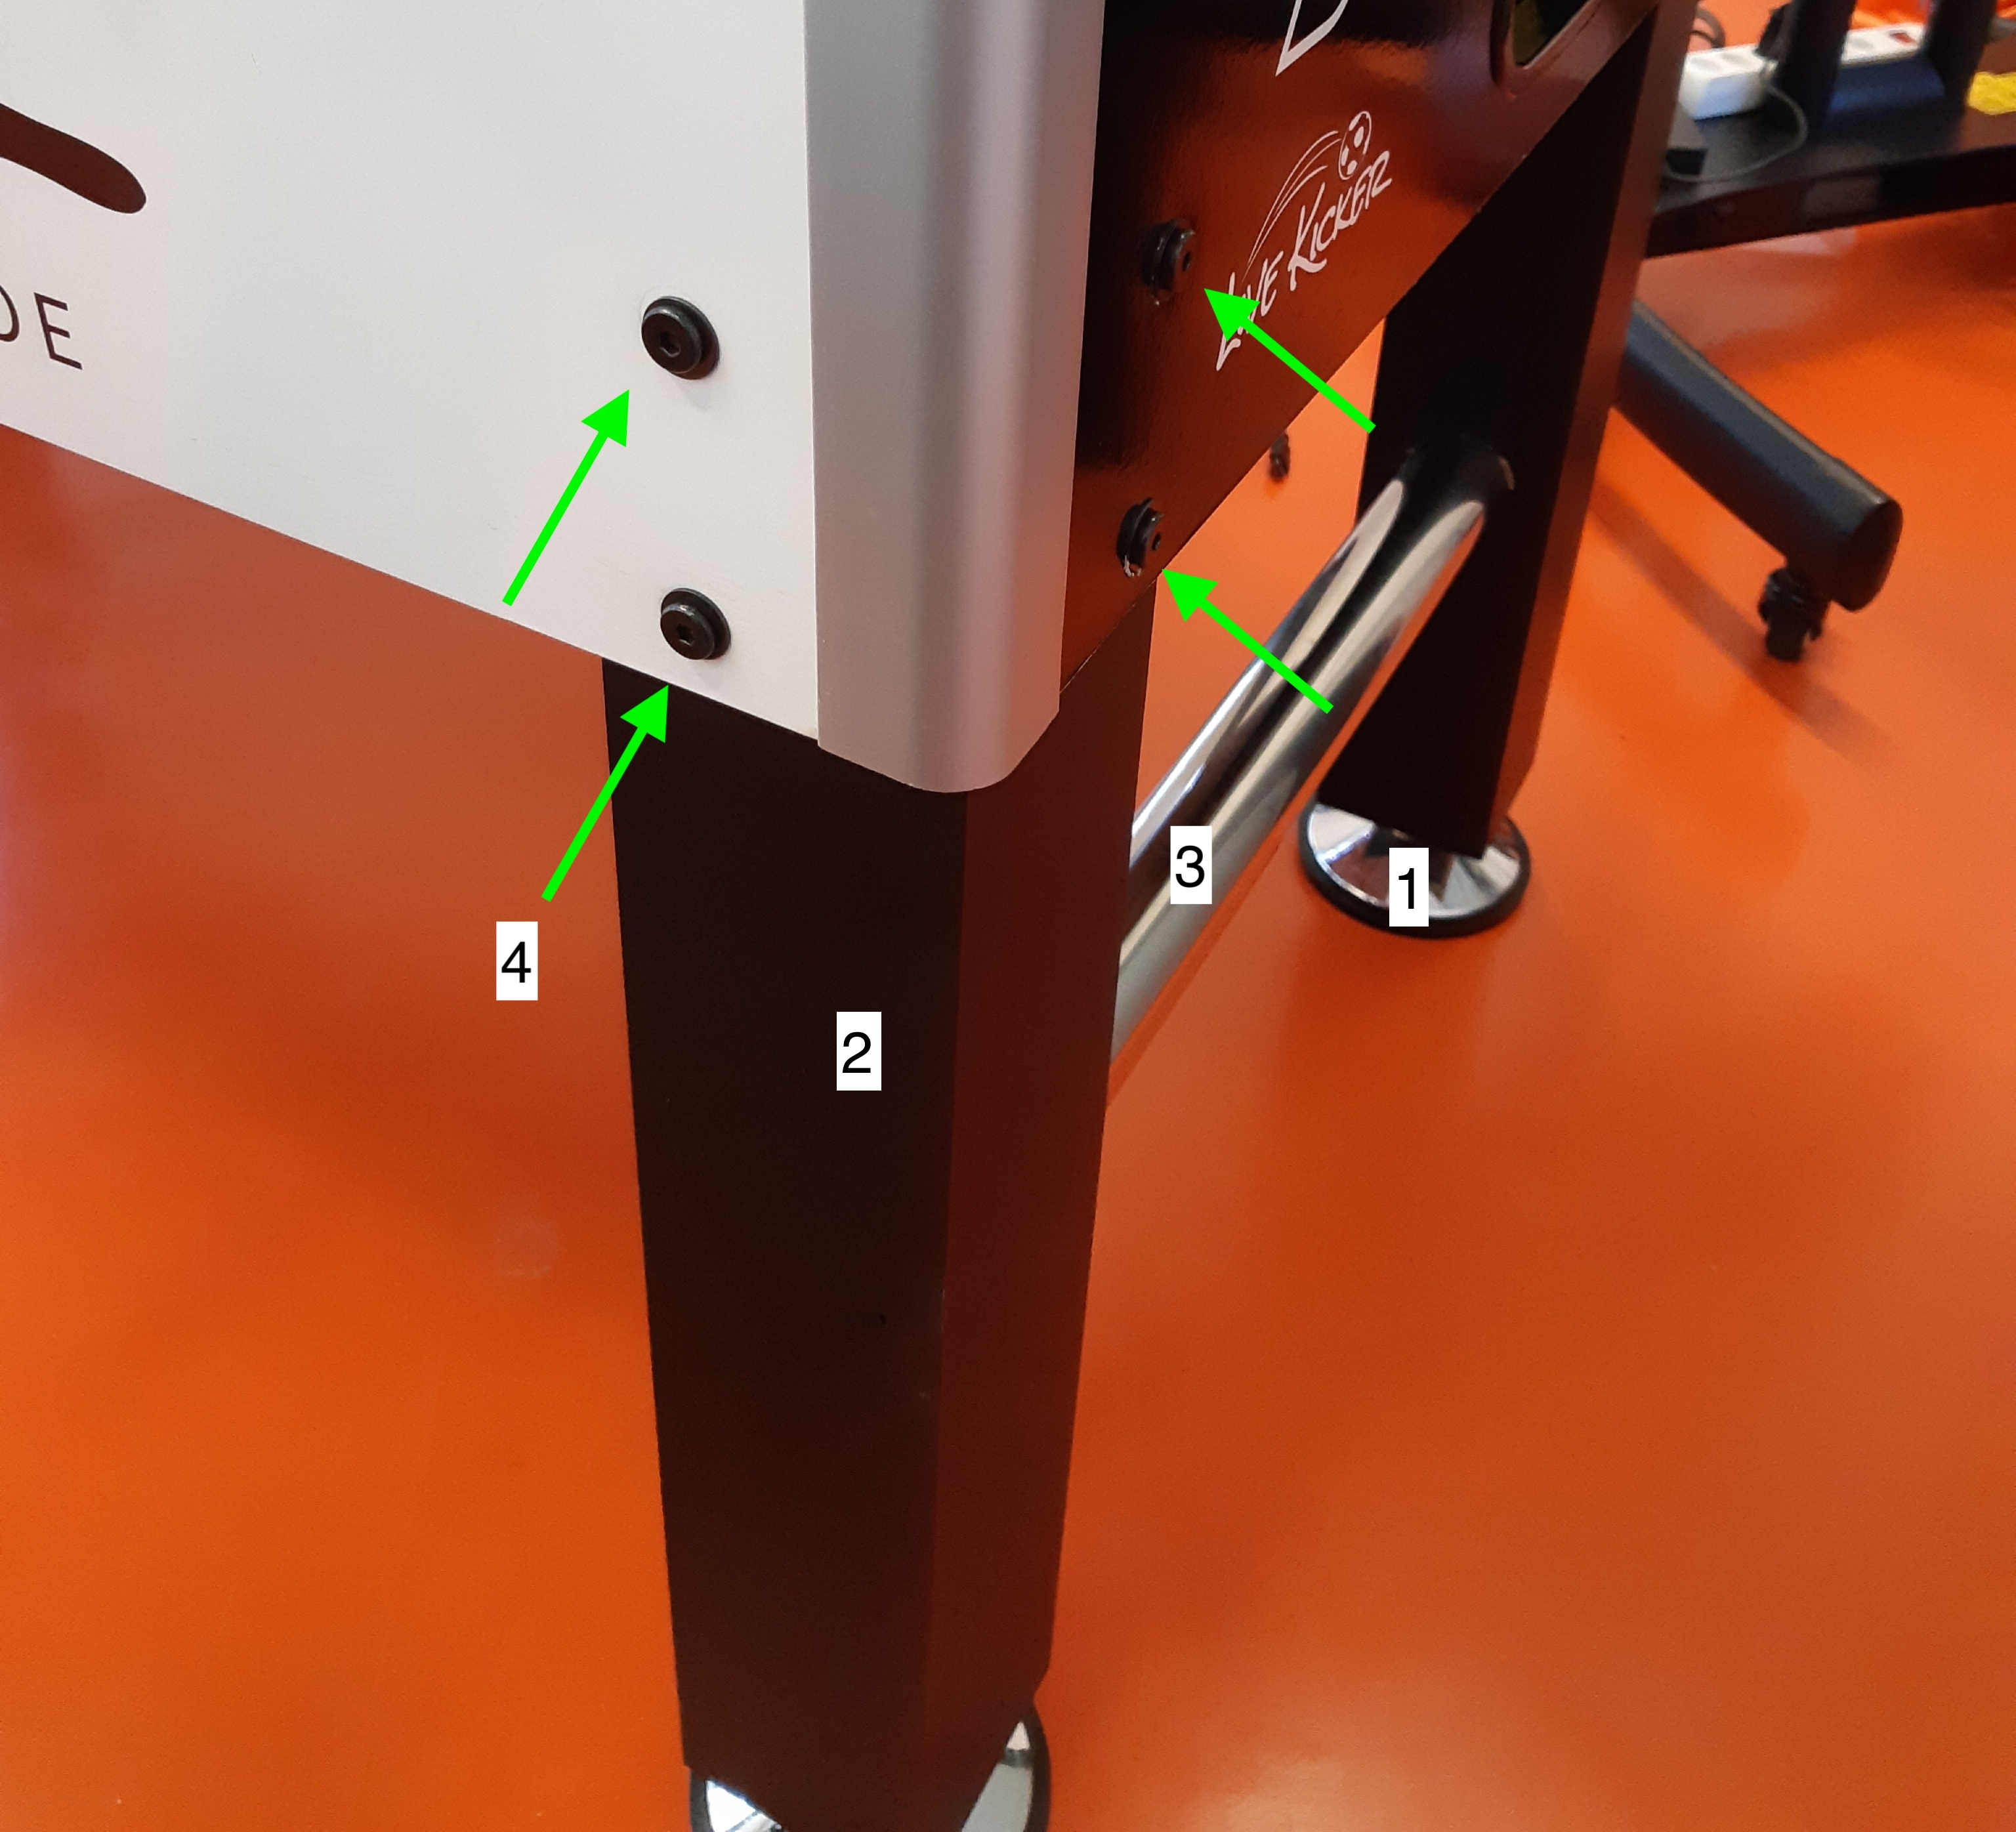
\includegraphics[width=0.9\textwidth]{img/screws.jpg}
        \end{figure}
        
        
      \subsection{Giocatori}
      
      Posizionare i giocatori secondo lo schema desiderato e fissarli in posizione. Per separarli, premere la linguetta sul lato destro e tirare delicatamente la parte inferiore.
      
      	\begin{figure}[H]
        		\begin{subfigure}{0.5\textwidth}
                \includegraphics[width=0.9\textwidth]{img/man1.jpg}
        \end{subfigure}
        \begin{subfigure}{0.5\textwidth}
                \includegraphics[width=0.9\textwidth]{img/man2.jpg}
         \end{subfigure}
	\end{figure}
		
		

\section{Utilizzo}

	Per iniziare a giocare, collegare la presa di corrente e aspettare qualche secondo. Dopo il tono di avvio, il tavolo sarà pronto all'uso.
	
	Ad ogni goal segnato, il tavolo si illuminerà brevemente con il colore della squadra corrispondente. Quando una delle due squadre raggiunge la vittoria (10 punti), il colore corrispondente lampeggia in continuo e i goal non vengono più conteggiati. È possibile annullare la vittoria in caso di un errore (vedi sotto).
	
	Per aggiustare manualmente il punteggio (in caso di errori di rilevamento), su ogni lato sono disponibili dei pulsanti per incrementare (\texttt{+}) o decrementare (\texttt{-}) manualmente il punteggio.
	
	Per cominciare una nuova partita, premere il tasto rosso (\texttt{Restart}).
	
	Per cambiare il colore o spegnere le luci, premere il tasto blu (\texttt{Lights}).
	
	\begin{figure}[H]
        \begin{subfigure}{0.5\textwidth}
                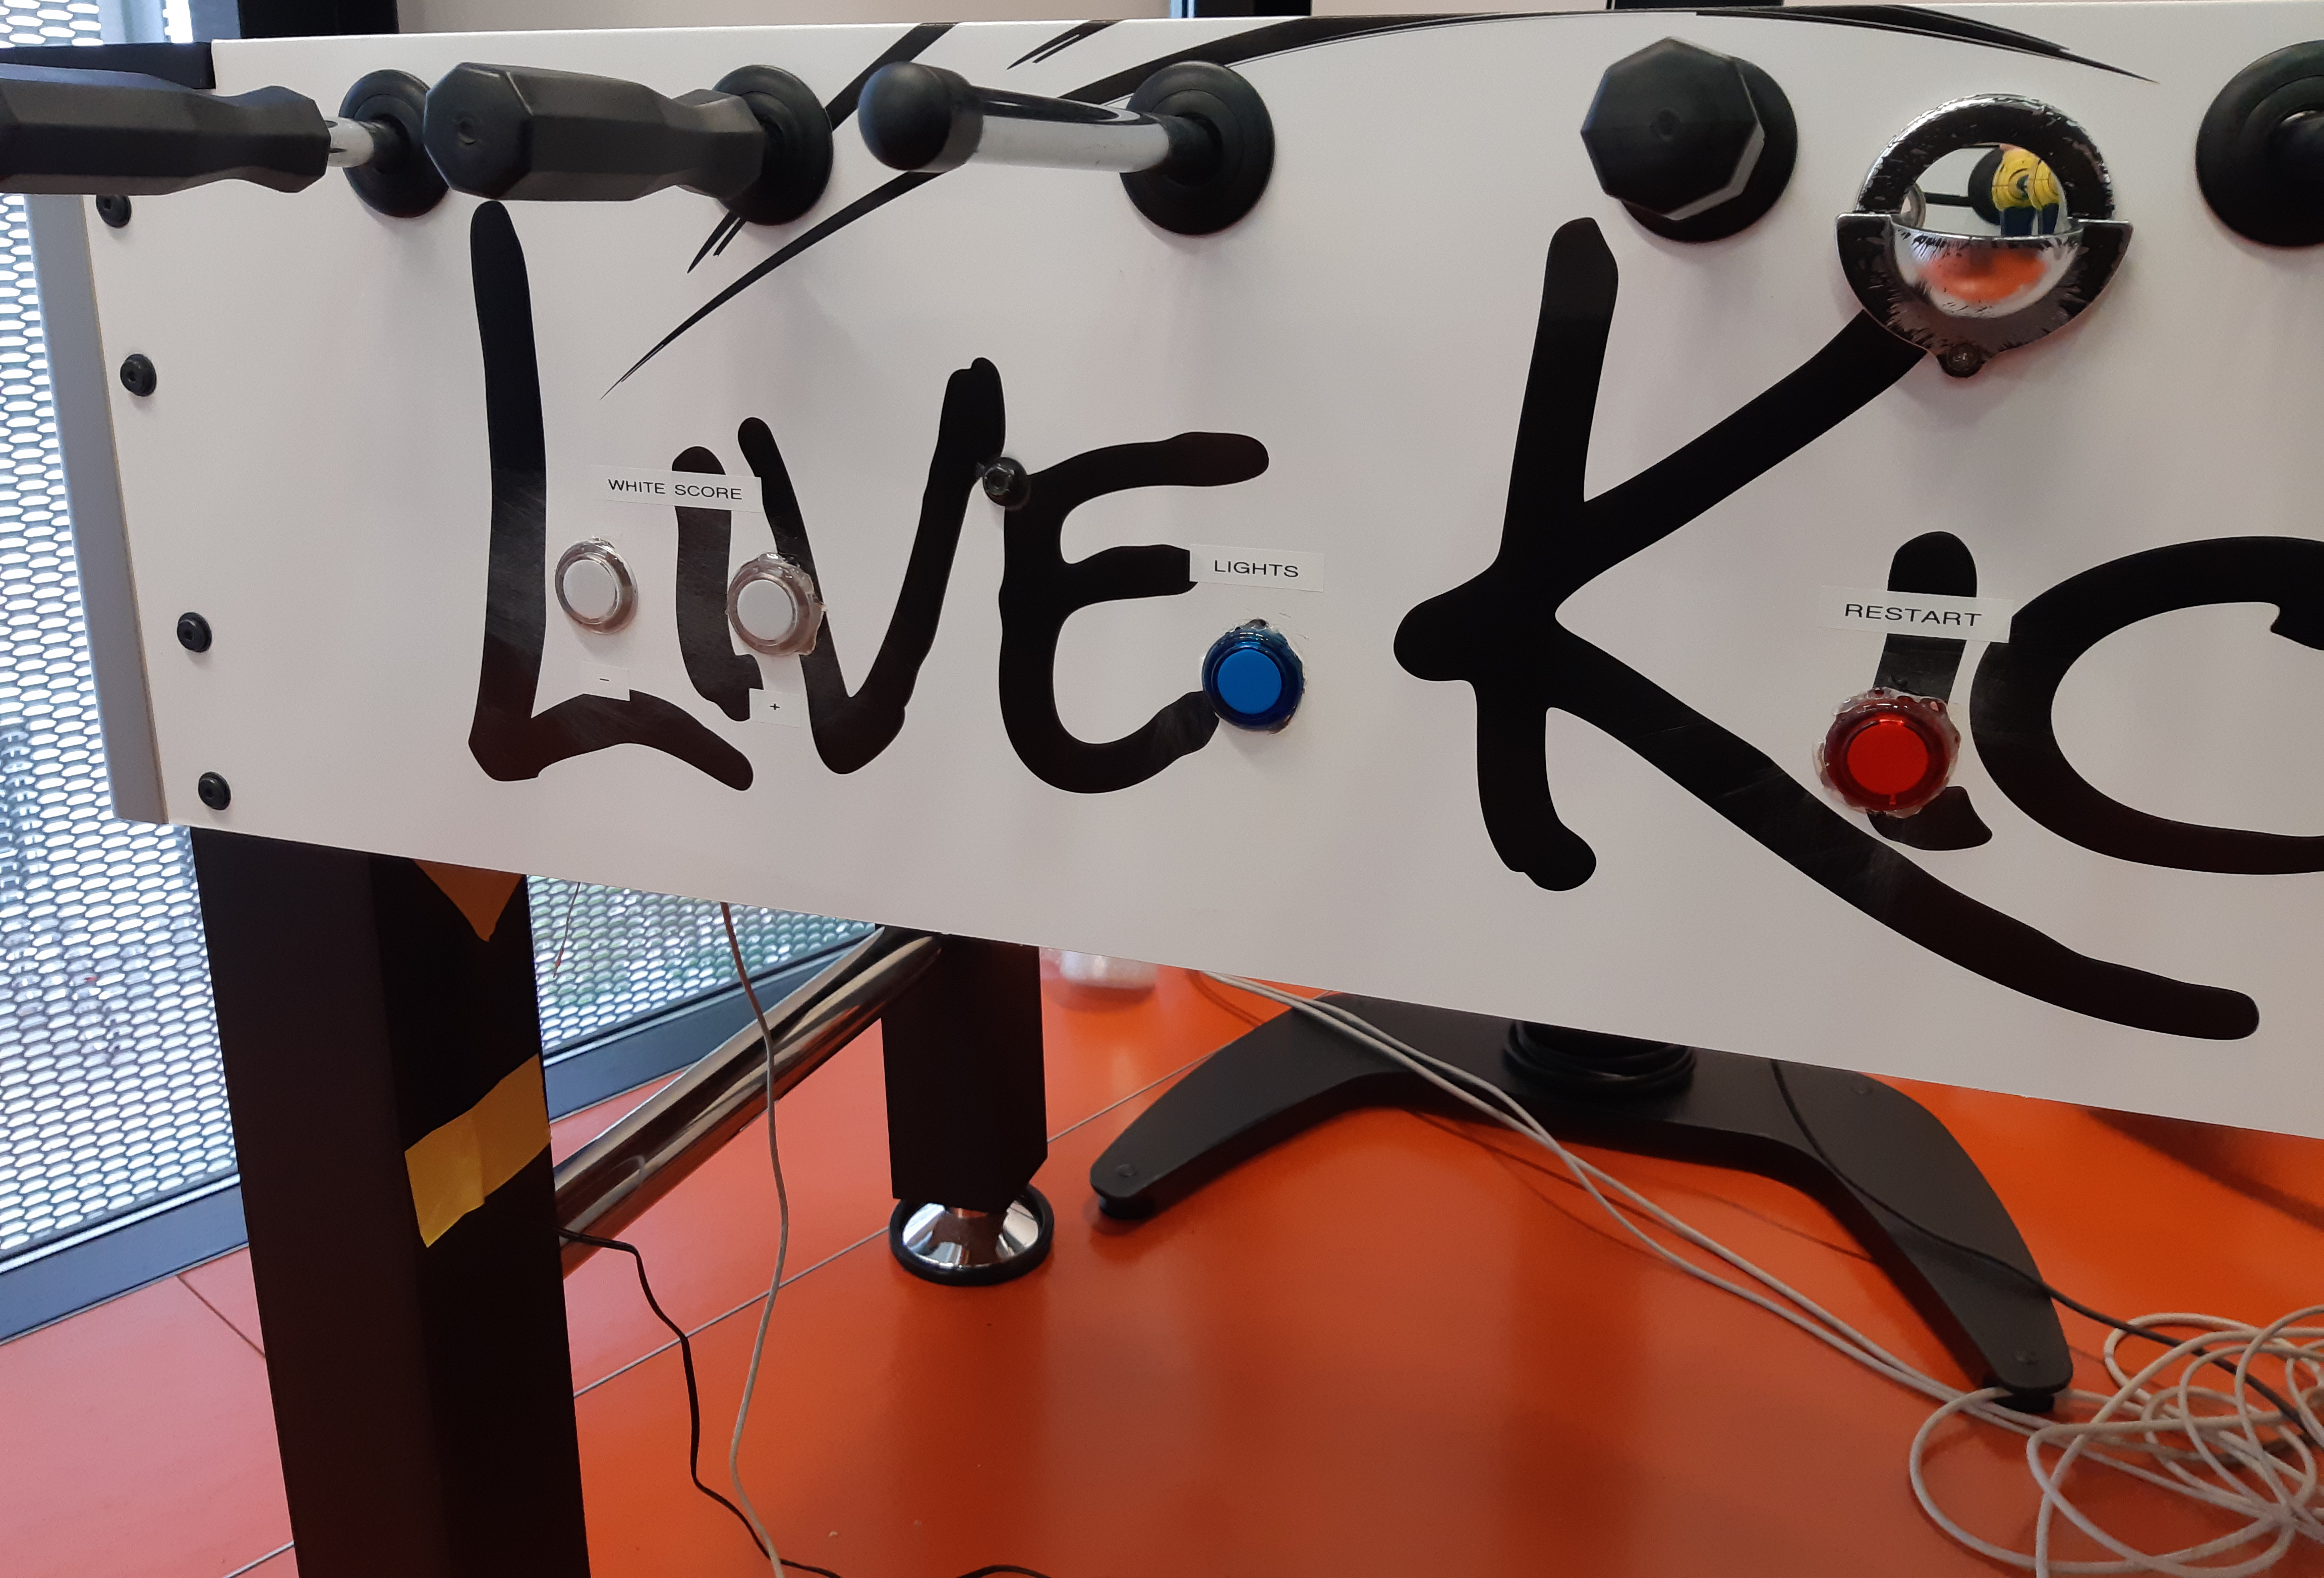
\includegraphics[width=0.9\textwidth]{img/btn_white.jpg}
                \caption*{I pulsanti per il team bianco}
        \end{subfigure}
        \begin{subfigure}{0.5\textwidth}
                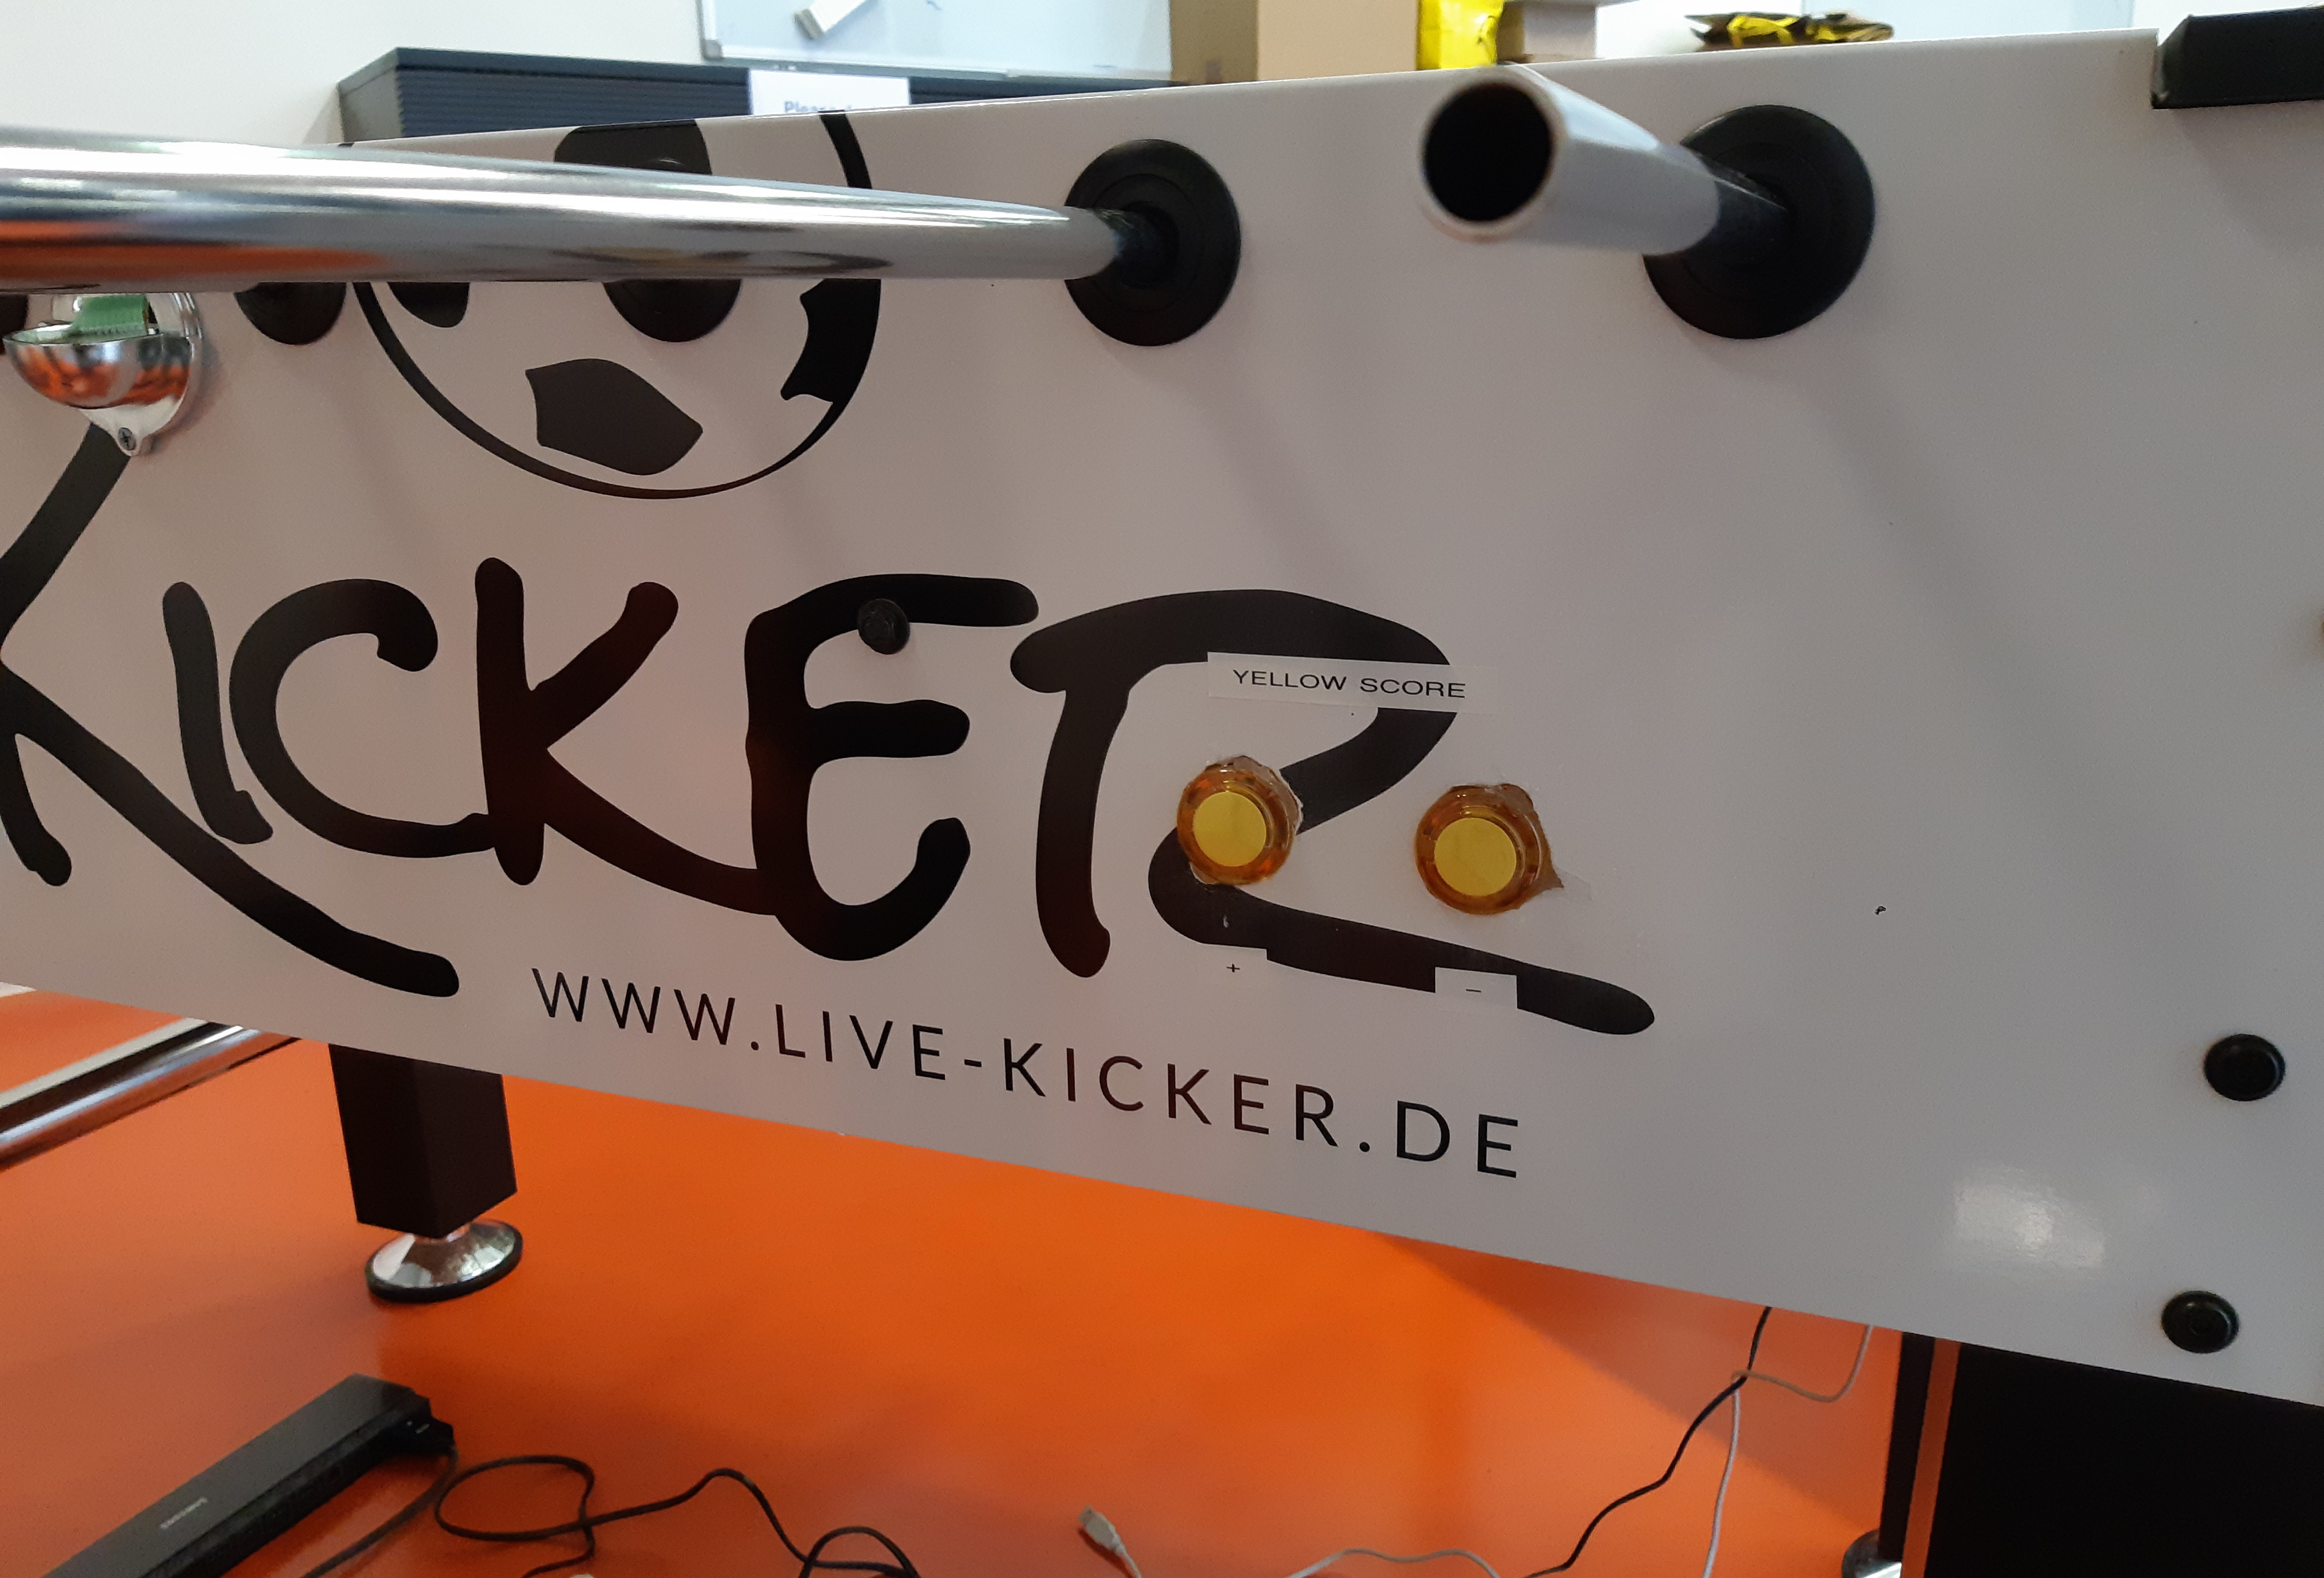
\includegraphics[width=0.9\textwidth]{img/btn_yellow.jpg}
                \caption*{I pulsanti per il team giallo}
         \end{subfigure}
	\end{figure}
	
	
	
\section{Circuito}

	Di seguito è una rappresentazione schematica del circuito: 
	
	\begin{figure}[H]
                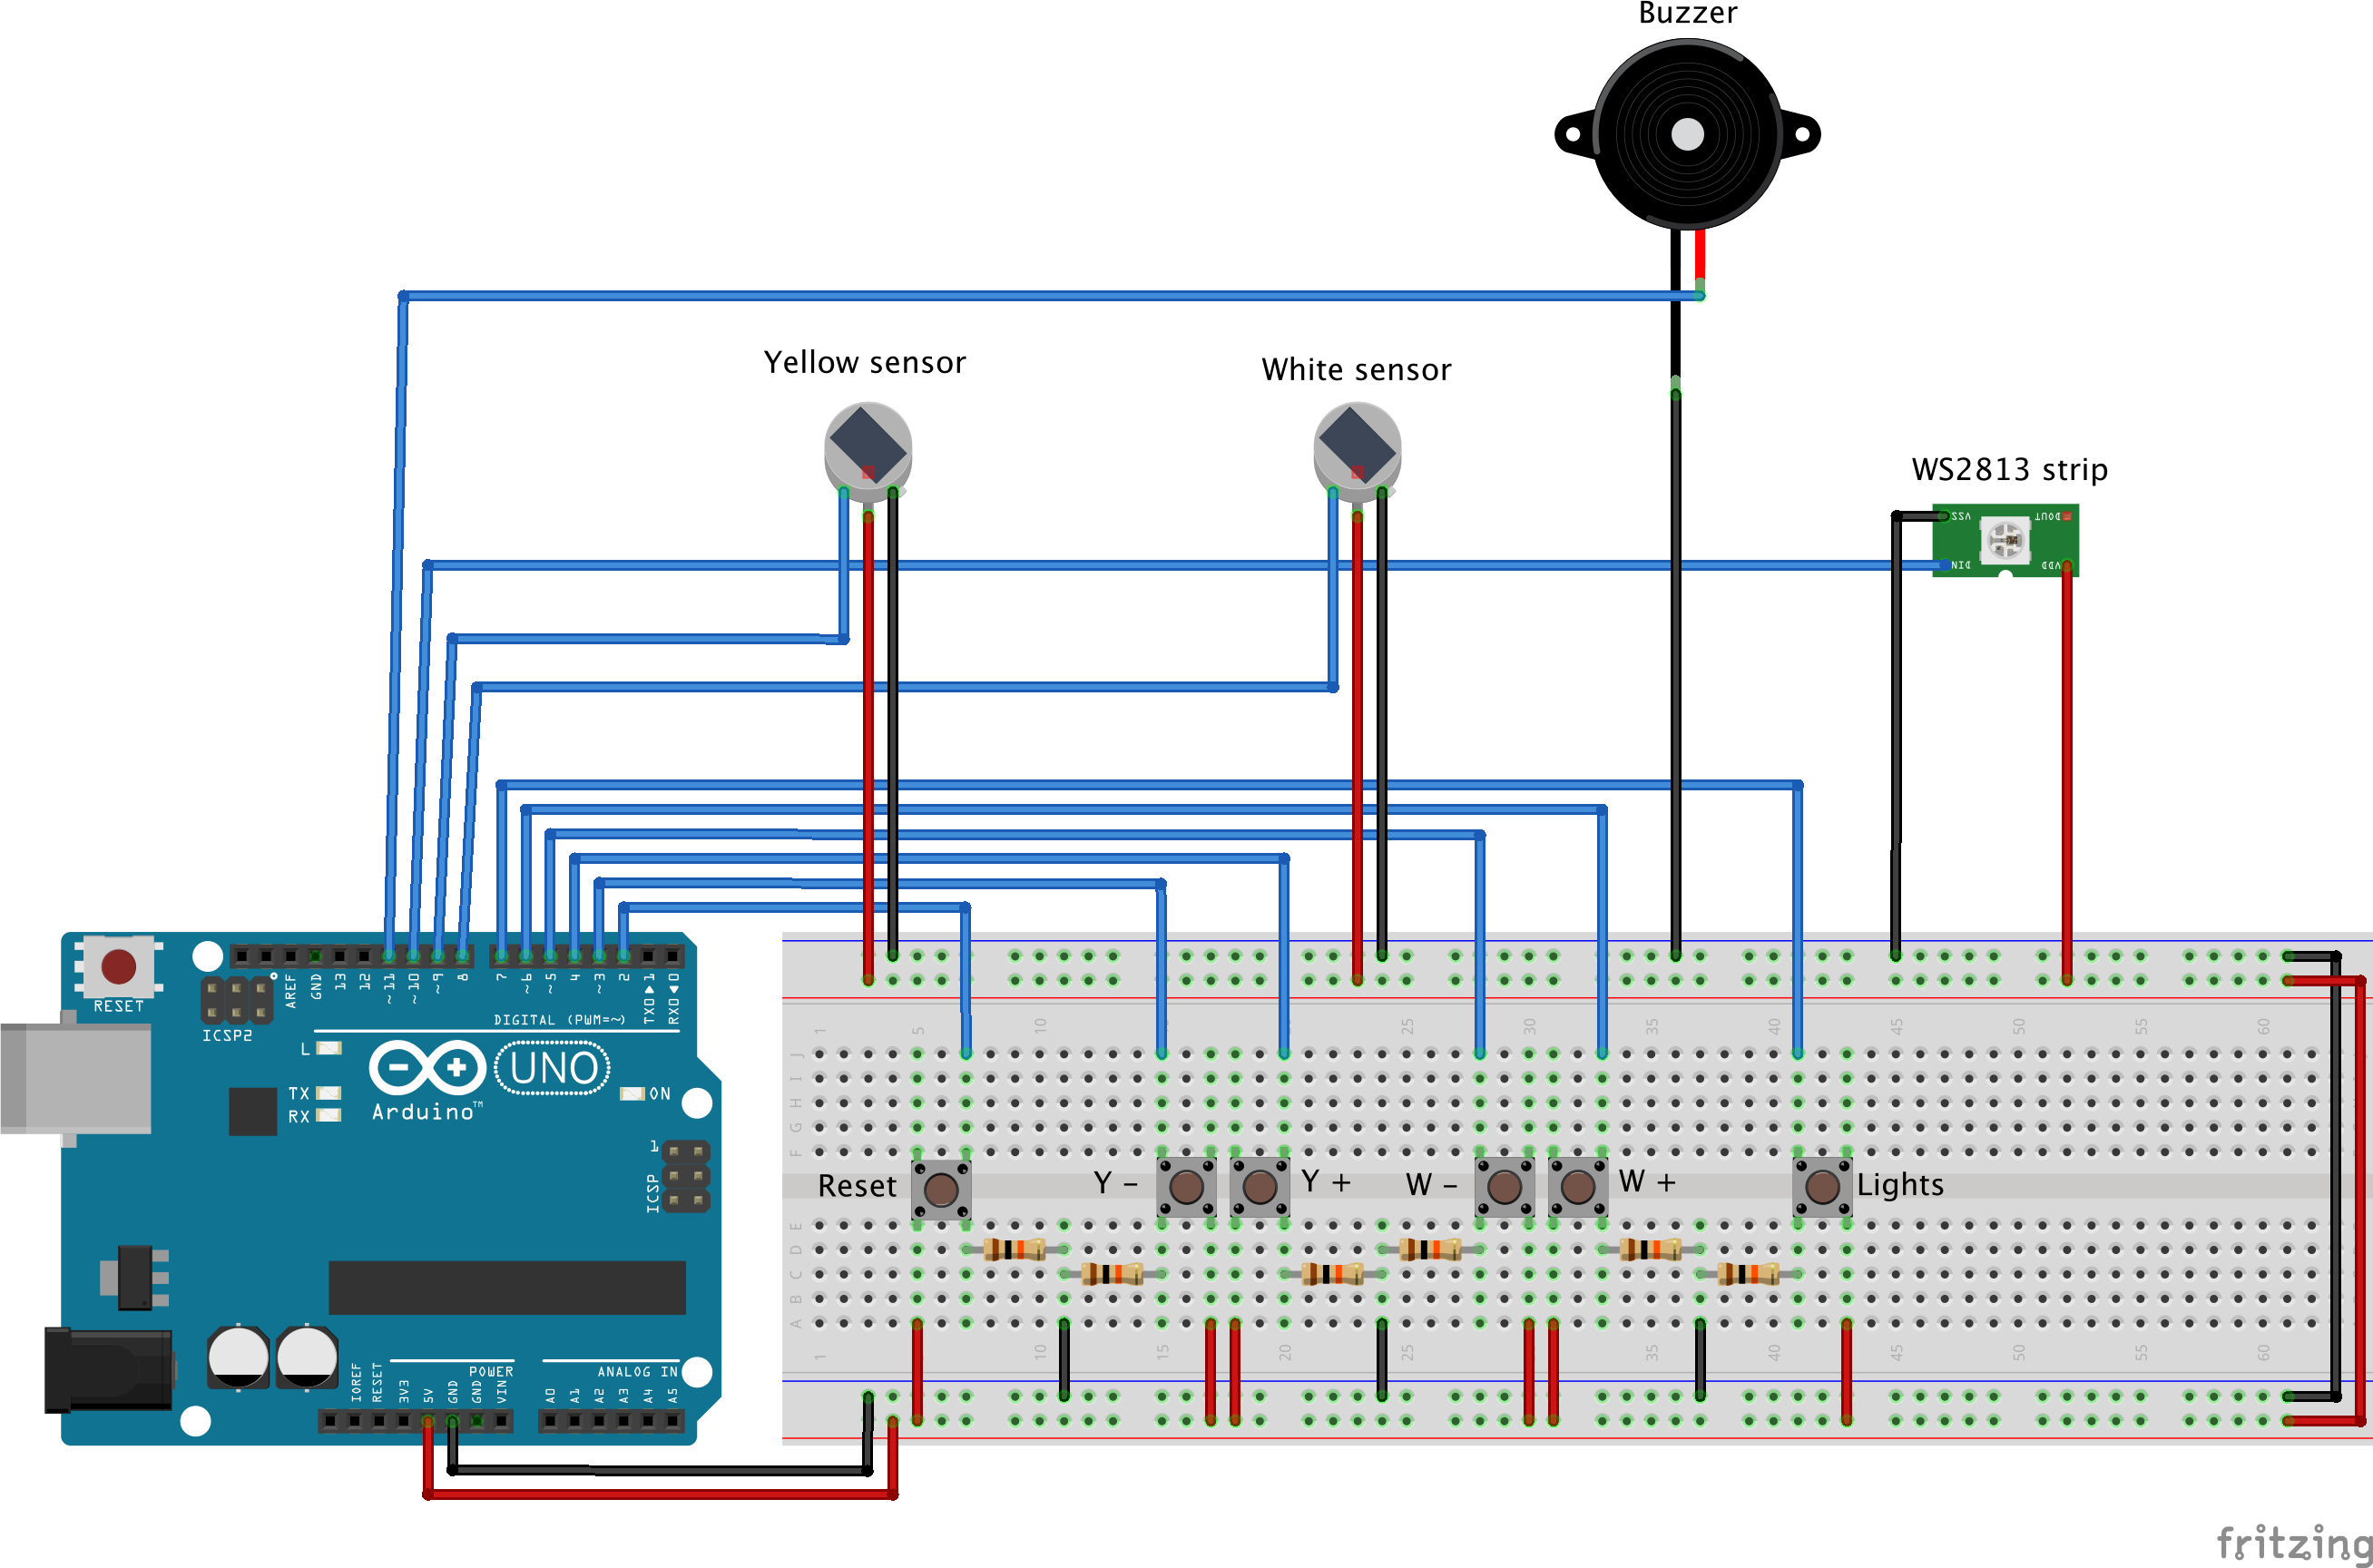
\includegraphics[width=\textwidth]{img/circuit.png}
        \end{figure}
	


\section{Codice}

	Il codice e la presente documentazione si trovano al seguente indirizzo: \url{https://github.com/USI-Showroom/TableFootballPlus}

\end{document}
